%\VignetteIndexEntry{faoswsFlag:A package to perform flag aggregation and much more}
%\VignetteEngine{knitr::knitr}
\documentclass[nojss]{jss}\usepackage[]{graphicx}\usepackage[]{color}
%% maxwidth is the original width if it is less than linewidth
%% otherwise use linewidth (to make sure the graphics do not exceed the margin)
\makeatletter
\def\maxwidth{ %
  \ifdim\Gin@nat@width>\linewidth
    \linewidth
  \else
    \Gin@nat@width
  \fi
}
\makeatother

\definecolor{fgcolor}{rgb}{0.345, 0.345, 0.345}
\newcommand{\hlnum}[1]{\textcolor[rgb]{0.686,0.059,0.569}{#1}}%
\newcommand{\hlstr}[1]{\textcolor[rgb]{0.192,0.494,0.8}{#1}}%
\newcommand{\hlcom}[1]{\textcolor[rgb]{0.678,0.584,0.686}{\textit{#1}}}%
\newcommand{\hlopt}[1]{\textcolor[rgb]{0,0,0}{#1}}%
\newcommand{\hlstd}[1]{\textcolor[rgb]{0.345,0.345,0.345}{#1}}%
\newcommand{\hlkwa}[1]{\textcolor[rgb]{0.161,0.373,0.58}{\textbf{#1}}}%
\newcommand{\hlkwb}[1]{\textcolor[rgb]{0.69,0.353,0.396}{#1}}%
\newcommand{\hlkwc}[1]{\textcolor[rgb]{0.333,0.667,0.333}{#1}}%
\newcommand{\hlkwd}[1]{\textcolor[rgb]{0.737,0.353,0.396}{\textbf{#1}}}%

\usepackage{framed}
\makeatletter
\newenvironment{kframe}{%
 \def\at@end@of@kframe{}%
 \ifinner\ifhmode%
  \def\at@end@of@kframe{\end{minipage}}%
  \begin{minipage}{\columnwidth}%
 \fi\fi%
 \def\FrameCommand##1{\hskip\@totalleftmargin \hskip-\fboxsep
 \colorbox{shadecolor}{##1}\hskip-\fboxsep
     % There is no \\@totalrightmargin, so:
     \hskip-\linewidth \hskip-\@totalleftmargin \hskip\columnwidth}%
 \MakeFramed {\advance\hsize-\width
   \@totalleftmargin\z@ \linewidth\hsize
   \@setminipage}}%
 {\par\unskip\endMakeFramed%
 \at@end@of@kframe}
\makeatother

\definecolor{shadecolor}{rgb}{.97, .97, .97}
\definecolor{messagecolor}{rgb}{0, 0, 0}
\definecolor{warningcolor}{rgb}{1, 0, 1}
\definecolor{errorcolor}{rgb}{1, 0, 0}
\newenvironment{knitrout}{}{} % an empty environment to be redefined in TeX

\usepackage{alltt}
\usepackage{url}
\usepackage[sc]{mathpazo}
\usepackage{geometry}
\geometry{verbose,tmargin=2.5cm,bmargin=2.5cm,lmargin=2.5cm,rmargin=2.5cm}
\setcounter{secnumdepth}{2}
\setcounter{tocdepth}{2}
\usepackage{breakurl}
\usepackage{hyperref}
\usepackage[ruled, vlined]{algorithm2e}
\usepackage{mathtools}
%% \usepackage{draftwatermark}
\usepackage{float}
\usepackage{placeins}
\usepackage{mathrsfs}
\usepackage{multirow}
%% \usepackage{mathbbm}
\DeclareMathOperator{\sgn}{sgn}
\DeclareMathOperator*{\argmax}{\arg\!\max}



\title{\bf faoswsFlag:A package to perform \\flag aggregation and much
  more}

\author{Michael. C. J. Kao\\ Food and Agriculture Organization \\ of
  the United Nations}

\Plainauthor{Michael. C. J. Kao} 

\Plaintitle{faoswsFlag:A package to manage flag aggregation}

\Shorttitle{Flag module}

\Abstract{ 

  This short documentation is intended to explain how observation
  flags are aggregated in the ESS Statistical Working System.
  
  The methodology and tools are presented step by step, with code
  examples and explanations.
  
  The paper also provide example of potential applications for
  integrating flag information.

}

\Keywords{meta data, flag aggregation}
\Plainkeywords{meta data, flag aggregation}

\Address{
  Michael. C. J. Kao\\
  Economics and Social Statistics Division (ESS)\\
  Economic and Social Development Department (ES)\\
  Food and Agriculture Organization of the United Nations (FAO)\\
  Viale delle Terme di Caracalla 00153 Rome, Italy\\
  E-mail: \email{michael.kao@fao.org}\\
  URL: \url{https://github.com/mkao006/sws_r_api/tree/master/faoswsFlag}
}
\IfFileExists{upquote.sty}{\usepackage{upquote}}{}
\begin{document}




\section{Introduction}
Lets start by loading the required library into R.

\begin{knitrout}
\definecolor{shadecolor}{rgb}{0.969, 0.969, 0.969}\color{fgcolor}\begin{kframe}
\begin{alltt}
\hlcom{## Load the required libraries}
\hlkwd{library}\hlstd{(faoswsFlag)}
\hlkwd{library}\hlstd{(ggplot2)}
\hlkwd{library}\hlstd{(splines)}
\end{alltt}
\end{kframe}
\end{knitrout}

Since the introduction of the new statistical working system, the old
symbol which reprents the collection and computation method of the
data is now represented by two separate flags.

The first, an observation flag which is a description of the
observation status, whether it be official, estimates or imputed
value. While on the other hand, the methodology flag contains
information of how it is collected or computed. It can be from survey,
questionnaire or it can be obtained as a balance or estimated through
statistical methodology.

The aim of this paper is to introduce a systematic way to aggregate
observation flags and further incorporate this piece of information in
to subsequent analysis.

Shown below is the corresponding table for the observation flags as of
\today{} outlined in Annex 5 of FAO Statistical Standards:

\begin{table}[h!]
  \begin{center}
    \caption{Description of the Observation flag}
    \begin{tabular}{|c|p{12cm}|}
      \hline
      Flags & Description\\
      \hline
      <blank> & Official Figure\\
      E & Estimates\\
      I & Imputed\\
      M & Missing\\
      T & Unofficial figure\\
      \hline
    \end{tabular}
  \end{center}  
\end{table}

The remaining of the paper is divided into three sections. First, we
show how to crate a table which holds the rank information required
for aggregation. The second part will illustrate how multiple flags
can be aggregated by using functions provided in the package. Finally,
the last section will present a simulated case how the use of these
data can help us build better models.


\section{Specification of a Mapping Table}

In order to compute aggregation of flags, one must convert the symbol
into a numerical type. The way this should be handled is assign a
value based on the amount of information quantity and the reliability
of the observation status.

Data obtained from reliable source should have a high information
content and thus should be assigned a high value, while data based on
human estimation should be assigned a low level of score to reflect
that the data is not directly observed and error may result as a case.

Shown below is the default weights table for the new statistical
working system.

\begin{knitrout}
\definecolor{shadecolor}{rgb}{0.969, 0.969, 0.969}\color{fgcolor}\begin{kframe}
\begin{alltt}
\hlcom{## Printed here is the default flag conversion table shipped with the}
\hlcom{## package.}
\hlstd{faoswsFlagTable}
\end{alltt}
\begin{verbatim}
##   flagObservationStatus flagObservationWeights
## 1                                         1.00
## 2                     T                   0.80
## 3                     E                   0.75
## 4                     I                   0.50
## 5                     M                   0.00
\end{verbatim}
\end{kframe}
\end{knitrout}

From this table, we have assigned 1 to official figure while 0 to
missing values. Albeit the arbitrary selection of the values, it
provides a rank of the information content which is necessary for the
computation of flag aggregation.

Flag tables can be created for each separate application depending on
the goal. For the aggregation of flag, only one restriction is applied
and that is the value of the weights are unique.


\section{Compute Flag Aggregation}

In this section, we take the computation of yield for example and
illustrate how to compute flag aggregation with the package. 

The value of yield is computed based on production and area harvested
which may come from different sources. Thus, when we compute a derived
statistic which is unobserved such as the yield; it is important that
the information quality reflect the lowest level that is used in the
computation. For a set of aggregation, the minimum of the set is taken
as the final observation flag.

A more concrete example is to say that we may have a production value
recorded from official survey (), while the area harvested was
collected from an unofficial external data base (T). Following this
principle, the resulting flag for yield should return (T) to reflect
the lower information content of the unofficial figure.


\begin{knitrout}
\definecolor{shadecolor}{rgb}{0.969, 0.969, 0.969}\color{fgcolor}\begin{kframe}
\begin{alltt}
\hlcom{## The function works just like sum(), with an optional arguement for}
\hlcom{## the flag table to be used.}
\hlkwd{aggregateObservationFlag}\hlstd{(}\hlstr{""}\hlstd{,} \hlstr{"T"}\hlstd{,} \hlkwc{flagTable} \hlstd{= faoswsFlagTable)}
\end{alltt}
\begin{verbatim}
## [1] "T"
\end{verbatim}
\end{kframe}
\end{knitrout}

\begin{knitrout}
\definecolor{shadecolor}{rgb}{0.969, 0.969, 0.969}\color{fgcolor}\begin{kframe}
\begin{alltt}
\hlcom{## Aggregation of multiple flag}

\hlcom{## Simulate flag for production}
\hlstd{simulatedProductionFlag} \hlkwb{=}
    \hlstd{faoswsFlagTable[}\hlkwd{sample}\hlstd{(}\hlnum{1}\hlopt{:}\hlkwd{NROW}\hlstd{(faoswsFlagTable),} \hlnum{10}\hlstd{,} \hlkwc{replace} \hlstd{=} \hlnum{TRUE}\hlstd{),}
                    \hlstr{"flagObservationStatus"}\hlstd{]}
\hlstd{simulatedProductionFlag}
\end{alltt}
\begin{verbatim}
##  [1] ""  "T" "T" "I" "E" "M" "T" "T" "M" "I"
\end{verbatim}
\begin{alltt}
\hlcom{## Simulated flag for area harvested}
\hlstd{simulatedAreaFlag} \hlkwb{=}
    \hlstd{faoswsFlagTable[}\hlkwd{sample}\hlstd{(}\hlnum{1}\hlopt{:}\hlkwd{NROW}\hlstd{(faoswsFlagTable),} \hlnum{10}\hlstd{,} \hlkwc{replace} \hlstd{=} \hlnum{TRUE}\hlstd{),}
                    \hlstr{"flagObservationStatus"}\hlstd{]}
\hlstd{simulatedAreaFlag}
\end{alltt}
\begin{verbatim}
##  [1] "I" "E" "M" "T" ""  "M" "T" "E" "T" "E"
\end{verbatim}
\begin{alltt}
\hlcom{## Now compute the aggregation of flag}
\hlkwd{aggregateObservationFlag}\hlstd{(simulatedProductionFlag, simulatedAreaFlag,}
                         \hlkwc{flagTable} \hlstd{= faoswsFlagTable)}
\end{alltt}
\begin{verbatim}
##  [1] "I" "E" "M" "I" "E" "M" "T" "E" "M" "I"
\end{verbatim}
\end{kframe}
\end{knitrout}


Currently, the weights of the flags are chosen as arbitrary mainly to
preserve a rank order based on expert judgement. Nevertheless, this
information can be estimated from the data and history of the flag as
we wil discuss more in the improvement section.



\section{Other Applications}
The converesion of the symbol to a numeric value has various advantage
than solely for the purpose of constructing aggregation. It can assist
subsequent modelling by identifying the quality of data and enable an
algorithm to take into account of the difference among various data
source.

For example, instead of fitting a linear regression by treating all
observation equally with the same source and identical quality, we can
estimate a weighted regression which gives more weight to data which
are of higher reliability.


\subsection{Robust Fitting to Anormalies}
The following artificial example illustrates how accounting for the
information source can result in a better fit and incorporate poor
data quality. The artificial data starts in 1991 and ends in 2014,
with all the observation collected as unofficial figure except the
last two which were estimated. For illustrative purpose, the values
were estimated by a poor algorithm and can be seen in the graph as
anormalies. The illustration shows how accounting for the anormalies
through the use of meta data can result in more robust model fitting
than as treating all data have the same information quality.

Figure below shows the value of simulated production with respect to
time, they are labelled by their corresponding flag. The fit of the
linear regression when all observation are treated equally is
illustrated in red. On the other hand, the blue line corresponds to
the fit of a weighted regression which gave less weight for the
suspicious point as it was marked as estimated (E) by the flag and
takes only half the weight of an official observation.

The dataset contains two flag, E and T which has weight of 0.4 and 0.8
respectively.

\begin{knitrout}
\definecolor{shadecolor}{rgb}{0.969, 0.969, 0.969}\color{fgcolor}\begin{kframe}
\begin{alltt}
\hlcom{## New table for simulation.}
\hlstd{simTable} \hlkwb{=} \hlstd{faoswsFlagTable}
\hlstd{simTable[simTable}\hlopt{$}\hlstd{flagObservationStatus} \hlopt{==} \hlstr{"E"}\hlstd{,}
         \hlstr{"flagObservationWeights"}\hlstd{]} \hlkwb{=} \hlnum{0.4}

\hlcom{## Simuate a data set which has a single point that was imputed badly }
\hlcom{## but still used for later analysis.}
\hlstd{x} \hlkwb{=} \hlnum{1991}\hlopt{:}\hlnum{2014}
\hlstd{y} \hlkwb{=} \hlnum{100} \hlopt{+} \hlnum{10} \hlopt{*} \hlstd{(x} \hlopt{-} \hlnum{1989}\hlstd{)} \hlopt{+} \hlkwd{rnorm}\hlstd{(}\hlkwd{length}\hlstd{(x),} \hlkwc{sd} \hlstd{=} \hlnum{30}\hlstd{)}
\hlstd{f} \hlkwb{=} \hlkwd{rep}\hlstd{(}\hlstr{"T"}\hlstd{,} \hlkwd{length}\hlstd{(x))}
\hlstd{y[}\hlnum{23}\hlopt{:}\hlnum{24}\hlstd{]} \hlkwb{=} \hlkwd{c}\hlstd{(}\hlnum{80}\hlstd{,} \hlnum{90}\hlstd{)}
\hlstd{f[}\hlnum{23}\hlopt{:}\hlnum{24}\hlstd{]} \hlkwb{=} \hlstr{"E"}
\hlstd{simulated.df} \hlkwb{=} \hlkwd{data.frame}\hlstd{(}\hlkwc{year} \hlstd{= x,} \hlkwc{simulatedProduction} \hlstd{= y,} \hlkwc{flag} \hlstd{= f)}

\hlcom{## Plot the data and show the two different fit when accounting for the }
\hlcom{## source and quality of information.}
\hlkwd{ggplot}\hlstd{(}\hlkwc{data} \hlstd{= simulated.df,}
       \hlkwd{aes}\hlstd{(}\hlkwc{x} \hlstd{= year,} \hlkwc{y} \hlstd{= simulatedProduction,} \hlkwc{label} \hlstd{= flag))} \hlopt{+}
    \hlkwd{geom_text}\hlstd{()} \hlopt{+}
    \hlkwd{geom_smooth}\hlstd{(}\hlkwc{method} \hlstd{=} \hlstr{"lm"}\hlstd{,} \hlkwc{formula} \hlstd{= y} \hlopt{~} \hlstd{x,}
                \hlkwc{data} \hlstd{= simulated.df,} \hlkwc{se} \hlstd{=} \hlnum{FALSE}\hlstd{,} \hlkwc{col} \hlstd{=} \hlstr{"red"}\hlstd{)} \hlopt{+}
    \hlkwd{geom_smooth}\hlstd{(}\hlkwc{method} \hlstd{=} \hlstr{"lm"}\hlstd{,} \hlkwc{formula} \hlstd{= y} \hlopt{~} \hlstd{x,}
                \hlkwd{aes}\hlstd{(}\hlkwc{weight} \hlstd{=} \hlkwd{flag2weight}\hlstd{(flag,} \hlkwc{flagTable} \hlstd{= simTable)),}
                \hlkwc{data} \hlstd{= simulated.df,} \hlkwc{se} \hlstd{=} \hlnum{FALSE}\hlstd{)}
\end{alltt}
\end{kframe}

{\centering 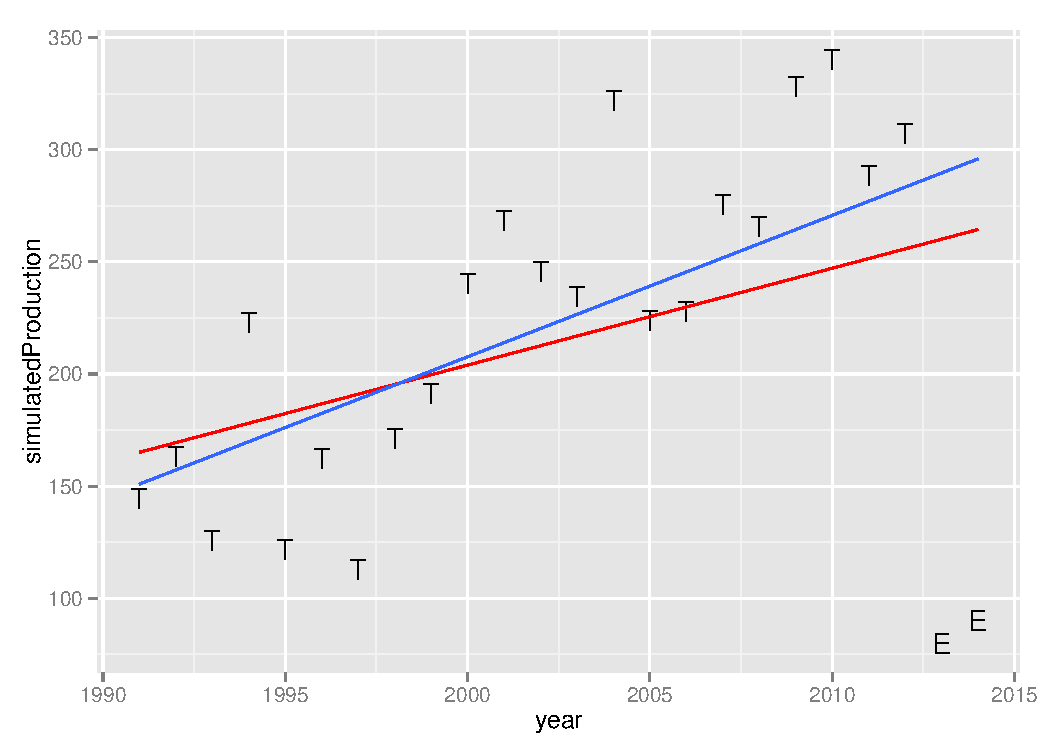
\includegraphics[width=\maxwidth]{figure/simulated-example} 

}



\end{knitrout}


\subsection{Weighted Source of Combination}

Another potential application of weight is for combining data from
various source to form an ensemble estimate.

Here we generate another artificial dataset for illustration. Assuming
we have two sources of data where each are collected on alternating
years and we would like to estimate the growth rate.

Plotted below is the simulated data, again the red is uniform weight
while the blue line represents the model which accounts for the
asymmetry of information. Since we trust data which are marked with T
with higher degree of believability, we can observe the estimated
growth curve is closer to the observed value marked as T.

\begin{knitrout}
\definecolor{shadecolor}{rgb}{0.969, 0.969, 0.969}\color{fgcolor}\begin{kframe}
\begin{alltt}
\hlstd{x} \hlkwb{=} \hlnum{1991}\hlopt{:}\hlnum{2014}
\hlstd{y} \hlkwb{=} \hlnum{100} \hlopt{+} \hlkwd{c}\hlstd{(}\hlnum{10}\hlstd{,} \hlnum{15}\hlstd{)} \hlopt{*} \hlstd{(x} \hlopt{-} \hlnum{1989}\hlstd{)}\hlopt{^}\hlnum{2} \hlopt{+} \hlkwd{rnorm}\hlstd{(}\hlkwd{length}\hlstd{(x),} \hlkwc{sd} \hlstd{=} \hlnum{20}\hlstd{)}
\hlstd{f} \hlkwb{=} \hlkwd{rep}\hlstd{(}\hlkwd{c}\hlstd{(}\hlstr{"E"}\hlstd{,} \hlstr{"T"}\hlstd{),} \hlkwd{length}\hlstd{(x)}\hlopt{/}\hlnum{2}\hlstd{)}
\hlstd{simulated.df} \hlkwb{=} \hlkwd{data.frame}\hlstd{(}\hlkwc{year} \hlstd{= x,} \hlkwc{simulatedProduction} \hlstd{= y,} \hlkwc{flag} \hlstd{= f)}

\hlcom{## Plot the data and show the two different fit when accounting for the }
\hlcom{## source and quality of information.}
\hlkwd{ggplot}\hlstd{(}\hlkwc{data} \hlstd{= simulated.df,}
       \hlkwd{aes}\hlstd{(}\hlkwc{x} \hlstd{= year,} \hlkwc{y} \hlstd{= simulatedProduction,} \hlkwc{label} \hlstd{= flag))} \hlopt{+}
    \hlkwd{geom_text}\hlstd{()} \hlopt{+}
    \hlkwd{geom_smooth}\hlstd{(}\hlkwc{method} \hlstd{=} \hlstr{"lm"}\hlstd{,} \hlkwc{formula} \hlstd{= y} \hlopt{~} \hlkwd{bs}\hlstd{(x),}
                \hlkwc{data} \hlstd{= simulated.df,} \hlkwc{se} \hlstd{=} \hlnum{FALSE}\hlstd{,} \hlkwc{col} \hlstd{=} \hlstr{"red"}\hlstd{)} \hlopt{+}
    \hlkwd{geom_smooth}\hlstd{(}\hlkwc{method} \hlstd{=} \hlstr{"lm"}\hlstd{,} \hlkwc{formula} \hlstd{= y} \hlopt{~} \hlkwd{bs}\hlstd{(x),}
                \hlkwd{aes}\hlstd{(}\hlkwc{weight} \hlstd{=} \hlkwd{flag2weight}\hlstd{(flag,} \hlkwc{flagTable} \hlstd{= simTable)),}
                \hlkwc{data} \hlstd{= simulated.df,} \hlkwc{se} \hlstd{=} \hlnum{FALSE}\hlstd{)}
\end{alltt}
\end{kframe}

{\centering 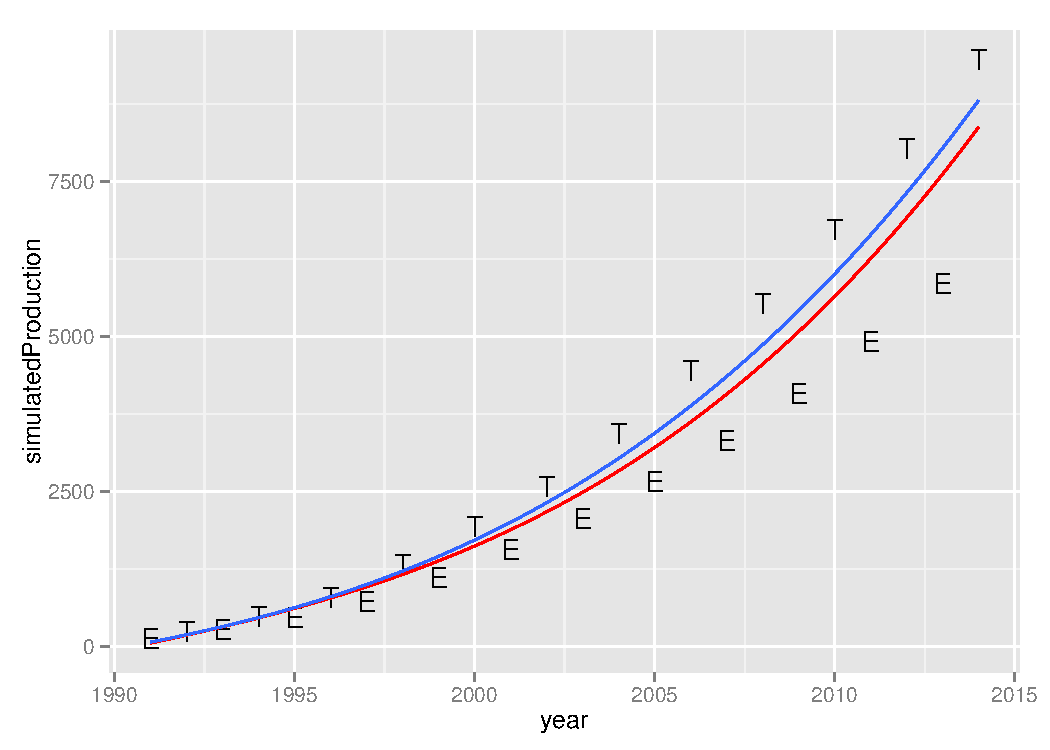
\includegraphics[width=\maxwidth]{figure/simulated-example2} 

}



\end{knitrout}

\section{Computing Weights}

To compute the weights objectively, we following the principle of
minimum discrimination information.\\

The information states that given derived information set, a new
distribution $q$ should be chosen which is as hard to discriminate
from the original distribution $p$ as possible; so that the new data
produces as small an information gain as possible.\\

In another word, if we have to choose another representation, the
information set which result in the least amount of information gain
or uncertainty should be chosen.\\

First of all, we take official figures as the desired
distribution. Then we can measured the information gain when we
replace data collection with imputed or estimated data.\\

The cross-entropy can be calculated as:

\begin{align*}
  \mathrm{H}(P, Q) &=  \mathrm{H}(P) + D_{\mathrm{KL}}(P \| Q)\\
  \intertext{Where}
  H(P) &= -\sum_{i} {p(x_i) \log p(x_i)},\\
  D_{\mathrm{KL}}(P\|Q) &= \sum_i \log\left(\frac{p(i)}{q(i)}\right) p(i).\\
\end{align*}



However, since the entropy of $H(x)$ would be the identical. We can
simple calculate the Kullback-Leibler Divergence
$D_{\mathrm{KL}}(P\|Q)$. After calculating the Kullback-Leibler
Divergence, we can compute the weight according to the information
gain.
  

\begin{equation*}
  \omega_i = \left\{
  \begin{array}{l r}
    1/(1 + D_{\mathrm{KL}}(P\|Q_i)) \quad \text{if $D_{\mathrm{KL}}(P\|Q_i) \ne 0$}\\
    1 - 1e^{-5} \, \, \, \, \quad \quad \quad \quad \quad \text{if $D_{\mathrm{KL}}(P\|Q_i) = 0$}
  \end{array} \right.
\end{equation*}


The following function shows how the weights can be computed from
historical information. This code is only executable when connected to
the intranet.

\begin{knitrout}
\definecolor{shadecolor}{rgb}{0.969, 0.969, 0.969}\color{fgcolor}\begin{kframe}
\begin{alltt}
\hlcom{## load the library}
\hlkwd{library}\hlstd{(faosws)}
\hlkwd{library}\hlstd{(faoswsExtra)}
\hlkwd{library}\hlstd{(faoswsFlag)}
\hlkwd{library}\hlstd{(data.table)}
\hlkwd{library}\hlstd{(FAOSTAT)}

\hlcom{## Set up the data query}
\hlstd{newPivot} \hlkwb{=} \hlkwd{c}\hlstd{(}
    \hlkwd{Pivoting}\hlstd{(}\hlkwc{code}\hlstd{=} \hlstr{"geographicAreaM49"}\hlstd{,} \hlkwc{ascending} \hlstd{=} \hlnum{TRUE}\hlstd{),}
    \hlkwd{Pivoting}\hlstd{(}\hlkwc{code}\hlstd{=} \hlstr{"measuredItemCPC"}\hlstd{,} \hlkwc{ascending} \hlstd{=} \hlnum{TRUE}\hlstd{),}
    \hlkwd{Pivoting}\hlstd{(}\hlkwc{code} \hlstd{=} \hlstr{"timePointYears"}\hlstd{,} \hlkwc{ascending} \hlstd{=} \hlnum{FALSE}\hlstd{),}
    \hlkwd{Pivoting}\hlstd{(}\hlkwc{code}\hlstd{=} \hlstr{"measuredElement"}\hlstd{,} \hlkwc{ascending} \hlstd{=} \hlnum{TRUE}\hlstd{)}
    \hlstd{)}

\hlstd{newKey} \hlkwb{=} \hlstd{swsContext.datasets}

\hlstd{getAllCountryCode} \hlkwb{=} \hlkwa{function}\hlstd{()\{}
    \hlcom{## 1062 is geographical world}
    \hlstd{keyTree} \hlkwb{=}
        \hlkwd{unique}\hlstd{(}\hlkwd{GetCodeTree}\hlstd{(}\hlkwc{domain} \hlstd{= swsContext.datasets[[}\hlnum{1}\hlstd{]]}\hlopt{@}\hlkwc{domain}\hlstd{,}
                           \hlkwc{dataset} \hlstd{= swsContext.datasets[[}\hlnum{1}\hlstd{]]}\hlopt{@}\hlkwc{dataset}\hlstd{,}
                           \hlkwc{dimension} \hlstd{=} \hlstr{"geographicAreaM49"}\hlstd{,}
                           \hlkwc{roots} \hlstd{=} \hlstr{"1062"}\hlstd{)}
               \hlstd{)}
    \hlstd{allCountryCode} \hlkwb{=}
        \hlkwd{unique}\hlstd{(}\hlkwd{adjacent2edge}\hlstd{(keyTree)}\hlopt{$}\hlstd{children)}
    \hlstd{allCountryCode[allCountryCode} \hlopt \hlstd{FAOcountryProfile}\hlopt{$}\hlstd{UN_CODE]}
\hlstd{\}}

\hlcom{## Create new key and download data, the history is for the whole}
\hlcom{## world since 1970 for wheat.}
\hlstd{newKey[[}\hlnum{1}\hlstd{]]}\hlopt{@}\hlkwc{dimensions}\hlopt{$}\hlstd{geographicAreaM49}\hlopt{@}\hlkwc{keys} \hlkwb{=} \hlkwd{getAllCountryCode}\hlstd{()}
\hlstd{newKey[[}\hlnum{1}\hlstd{]]}\hlopt{@}\hlkwc{dimensions}\hlopt{$}\hlstd{timePointYears}\hlopt{@}\hlkwc{keys} \hlkwb{=} \hlkwd{as.character}\hlstd{(}\hlnum{1970}\hlopt{:}\hlnum{2013}\hlstd{)}
\hlstd{newKey[[}\hlnum{1}\hlstd{]]}\hlopt{@}\hlkwc{dimensions}\hlopt{$}\hlstd{measuredItemCPC}\hlopt{@}\hlkwc{keys} \hlkwb{=} \hlstr{"0111"}

\hlcom{## Compute the table}
\hlstd{history} \hlkwb{=} \hlkwd{GetHistory}\hlstd{(newKey[[}\hlnum{1}\hlstd{]], newPivot)}
\hlstd{history[, timePointYears} \hlkwb{:=} \hlkwd{as.numeric}\hlstd{(timePointYears)]}
\hlstd{obsTable} \hlkwb{=} \hlkwd{computeFlagWeight}\hlstd{(history,} \hlkwc{method} \hlstd{=} \hlstr{"entropy"}\hlstd{)}
\end{alltt}
\end{kframe}
\end{knitrout}



%% \section{Further Improvements}
%% Currently, the method is only implement to perform flag
%% aggregation. Nevertheless, we would like to extend the possibility to
%% what has been demonstrated in the application section. In order to
%% achieve this, we would need a methodology allowing us to assign a
%% weight automatically and objectively.

%% Two method are being investigated, the first is to use official figure
%% as the benchmark and measure the loss in information through the use
%% of entropy. The greater the loss in information, the lower the weight
%% should be. This however, requires us to assume that the official
%% figure is of highest quality. On the other hand, the second
%% methodology does not make this assumption. Rather, it computes the
%% similarity between values of different flag then assign weights
%% according to the similarity. The rational of this approach is that the
%% data source which are close to what we want to measure will also be
%% close to data sources measured differently. This is similary to
%% finding the centroid which minimizes the within cluster sums of
%% variance.


\end{document}
